% Owner: Khalid  |  Task: T10  |  Drafted by ORCA agents, finalised by the owner.
% Rules: prose only; every claim cited with \citet/\citep to a literature/sources.yaml record id;
% compare methods (G6); strengths/weaknesses/applicability (G8). See tasks/todo.md.
% Every update rule below was checked against the cited paper's PDF (2026-11-07); equation
% numbers are given in comments next to each rule.
\section{Multi-Objective Optimization: A Primer}
\label{sec:moo}

A distillation loss is almost always a sum of a supervised task loss and one or more terms that
pull the student towards the teacher. This section sets out the multi-objective optimisation (MOO)
vocabulary that \S\ref{sec:kd_moo} needs, restricted to first-order rules that pick one update
direction from per-objective gradients; \citet{chen2026gradmoo} survey the wider field.

\paragraph{Pareto optimality and stationarity.}
Consider $K$ differentiable losses $L_1,\dots,L_K$ of shared parameters $\theta$, with
gradients $g_i=\nabla_\theta L_i(\theta)$. A point $\theta^\star$ is Pareto optimal when no other
point lowers one loss without raising another; gradient methods target the local notion of
\emph{Pareto stationarity}, where some convex combination of the gradients vanishes, $\sum_i\alpha_i g_i=0$ with $\alpha_i\ge0$ and
$\sum_i\alpha_i=1$. Every Pareto optimal point is Pareto stationary but not conversely
\citep{sener2018mgda}. Away from such points a direction $d$ exists with $g_i^\top d>0$ for every
$i$, so a small step along $-d$ lowers all losses; the rules below differ in which such direction they
pick and what they do when none exists.
% sener2018mgda Sec. 3.1, KKT conditions and the remark that Pareto optimal => Pareto stationary.

\paragraph{Linear scalarisation.}
The default in distillation is the weighted sum $L=\sum_i w_iL_i$ with fixed $w_i\ge0$, whose
gradient is $\sum_i w_ig_i$, at one backward pass. As the weights vary it reaches only the convex
part of the Pareto front \citep{gong2021dbgd}, and its direction follows raw gradient norms, so a
much larger gradient dominates unless the weights are retuned. Whether this matters in practice is
contested (\S\ref{sec:kd_moo_critical}).
% gong2021dbgd Sec. 1: "(2) can only capture the convex envelop of the Pareto front".

\subsection{Symmetric rules}
\label{sec:moo_symmetric}

The first family, designed for multi-task learning, treats all objectives alike: permuting the
losses does not change the update.

\paragraph{MGDA.}
\citet{sener2018mgda} cast multi-task learning as MOO with the multiple-gradient descent
algorithm (MGDA), which picks the minimum-norm point of the convex hull of the gradients,
$\min_{\alpha\in\Delta}\|\sum_i\alpha_ig_i\|_2^2$. The result is either zero, which certifies
Pareto stationarity, or a direction that decreases every loss. For two objectives the weight
has a closed form, $\hat\alpha=\big[(g_2-g_1)^\top g_2/\|g_1-g_2\|^2\big]_{[0,1]}$; for more
objectives, Frank--Wolfe; MGDA-UB takes gradients at a shared representation to need one backward
pass. Two-objective MGDA favours the \emph{smaller} gradient (an interior minimiser has equal inner
products with both), so with a large task and a small distillation gradient it moves mostly along
distillation (Fig.~\ref{fig:moo_geometry}). It suits problems where no objective may be sacrificed,
not ones where one matters more.
% sener2018mgda Eq. (3) (min-norm problem), Eq. (4) (two-task closed form, clipped to [0,1]),
% Sec. 3.2 / Alg. 2 (Frank-Wolfe), Sec. 3.3 (MGDA-UB, gradients w.r.t. the shared representation Z).

\paragraph{PCGrad.}
\citet{yu2020pcgrad} keep each task gradient but edit it when it conflicts with another.
If $g_i^\top g_j<0$, PCGrad replaces $g_i$ by its projection onto the normal plane of $g_j$,
$g_i\leftarrow g_i-\frac{g_i^\top g_j}{\|g_j\|^2}g_j$. It repeats this for every other task in
random order and sums the results. Unlike MGDA it leaves non-conflicting gradients untouched and
keeps the scale of the sum; it needs one backward pass per objective and gives no priority, so with
two objectives the task gradient loses its distillation component as much as the reverse.
% yu2020pcgrad Alg. 1 (lines 5-8) and Sec. 2.2 projection formula.

\paragraph{CAGrad.}
\citet{liu2021cagrad} seek, within a ball around the average gradient $g_0$, the direction that
most improves the worst-off objective:
$\max_d\min_i\langle g_i,d\rangle$ subject to $\|d-g_0\|\le c\|g_0\|$. The dual is a problem over
the simplex, $\min_{w\in\Delta}g_w^\top g_0+\sqrt{\phi}\|g_w\|$ with $\phi=c^2\|g_0\|^2$, and the
update is $d=g_0+\frac{\sqrt\phi}{\|g_w\|}g_w$. With $c=0$ CAGrad is plain gradient descent on the
average loss. As $c$ grows the authors show it approaches MGDA. The radius $c$ interpolates
between the weighted sum and MGDA, and CAGrad
inherits MGDA's symmetry and per-objective backward passes, and adds one hyperparameter.
% liu2021cagrad Eq. (3) (primal), Alg. 1 (dual over the simplex and the update), Sec. 4 Q2
% (recovers GD at c = 0 and MGDA as c grows).

\paragraph{Other symmetric rules.}
Nash-MTL solves a bargaining game, $G^\top G\alpha=1/\alpha$, whose solution is invariant to
rescaling any one loss but needs an iterative solver on top of $K$ backward passes
\citep{navon2022nashmtl}; FAMO applies the MGDA problem to log-loss gradients but amortises the
weights from observed loss changes, reaching MGDA-like balancing at one backward pass with weights
that lag a step \citep{liu2023famo}; and GradNorm and uncertainty weighting only retune scalar
weights, from gradient-norm targets and learned task noise respectively, so they address scale
imbalance but not conflict \citep{chen2018gradnorm,kendall2018uncertainty}.
% navon2022nashmtl Claim 3.1 (G^T G alpha = 1/alpha), Sec. 3 (scale-invariance axiom).
% liu2023famo Prop. 3.1 / Eq. (6) (dual = min-norm on grad log losses), Sec. 3.2 (amortised O(1) update).
% chen2018gradnorm Eq. (1)-(2); kendall2018uncertainty Eq. (7).

\subsection{Priority, lexicographic and constrained rules}
\label{sec:moo_priority}

The second family drops symmetry: one objective is primary and the others are constraints, which
matches the usual reading of distillation, where the student must fit the labels and the teacher
is useful but fallible. Each rule finds the direction closest to a reference gradient subject to
linear inequalities on the others; they differ in the reference, the required progress, and the
scaling.
DBGD minimises $\|\nabla f-v\|^2$ subject to $\nabla g^\top v\ge\phi(\theta)$, with closed form
$v=\nabla f+\lambda\nabla g$ and a barrier that forces progress on $g$ until its target is met; it
has continuous-time non-convex convergence results, and the authors argue a tuned weighted sum
cannot solve the constrained problem when the duality gap is non-zero \citep{gong2021dbgd}.
GEM and A-GEM, from continual learning, project the new-task gradient so that earlier-task
gradients do not get worse, i.e.\ with zero required progress \citep{lopezpaz2017gem,chaudhry2019agem}.
PNGD stays close to an external criterion $\nabla F$ with one scheduled margin on all losses
\citep{ye2022pngd}, and AuxiNash learns a preference vector over Nash-MTL's bargaining solution, so
its priority is learned and the main task's progress is not guaranteed \citep{shamsian2023auxinash}.
% gong2021dbgd Eq. (6), Eq. (4)/Alg. 1, Eq. (8), Sec. 3.4. lopezpaz2017gem Eq. (8), (11); chaudhry2019agem Eq. (10)-(11).
% ye2022pngd Eq. (7). shamsian2023auxinash Sec. 4.1, 4.2.

\paragraph{PCD.}
Priority-constrained descent \citep{varam2026pcd} rescales each gradient by an EMA of its norm and
solves $\min_{\tilde d}\tfrac12\|\tilde d-\tilde g_1\|^2$ subject to
$\tilde g_j^\top\tilde d\ge\tau\|\tilde g_j\|^2$; for two objectives,
$\tilde d^\star=\tilde g_1+\max\big(0,\tau-\tilde g_1^\top\tilde g_2/\|\tilde g_2\|^2\big)\tilde g_2$,
rescaled to the primary gradient norm, with no correction when the constraint already holds.
The authors say the program is not new (DBGD at $K=2$; A-GEM at $\tau=0$); they add the
normalisation, which makes $\tau$ scale-free, and a general-$K$ analysis. Each secondary makes
first-order progress, but the primary is not guaranteed to descend under strong conflict, no
convergence theorem covers the deployed algorithm, and, unlike AuxiNash, the priority is fixed
rather than learned. Its evidence comes from pruning and low-rank compression, not distillation.
% varam2026pcd Def. 4.1 / Eq. (4), Def. 4.5, Cor. 4.6 / Eq. (14), Alg. 1, Sec. 4.1, Sec. 2,
% Prop. 4.4, Prop. 4.7 (primary descent only if 1 + tau c - c^2 > 0), Sec. 4.8.

\subsection{The two families side by side}

\begin{figure}[t]
\centering
\resizebox{0.6\linewidth}{!}{% Generated by paper/survey/figures/moo_geometry.py -- do not edit by hand.
% g1 = [2.0, 0.5], g2 = [-0.5, 0.8], CAGrad c = 0.5, PCD tau = 0.5
% Weighted sum: (0.7500,0.6500)
% MGDA: (0.0875,0.7295)
% PCGrad: (1.4453,1.9099)
% CAGrad: (0.4870,1.0708)
% PCD: (1.4129,1.4393)
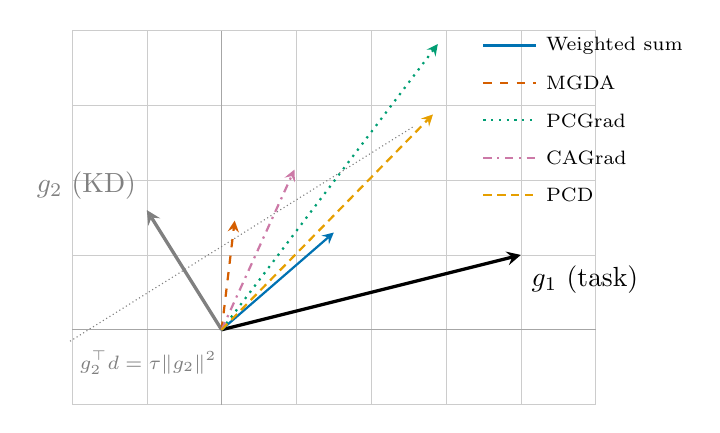
\begin{tikzpicture}[scale=1.9,>=stealth]
\draw[gray!40,very thin] (-1,-0.5) grid[step=0.5] (2.5,2);
\draw[gray!70] (-1,0) -- (2.5,0); \draw[gray!70] (0,-0.5) -- (0,2);
\draw[densely dotted,gray] (-1.0132,-0.0770) node[below right,font=\scriptsize] {$g_2^\top d=\tau\|g_2\|^2$} -- (1.2764,1.3540);
\draw[->,very thick,black] (0,0) -- (2.0000,0.5000) node[below right] {$g_1$ (task)};
\draw[->,very thick,gray] (0,0) -- (-0.5000,0.8000) node[above left] {$g_2$ (KD)};
\draw[->,thick,color={rgb,255:red,0;green,114;blue,178},solid] (0,0) -- (0.7500,0.6500);
\draw[->,thick,color={rgb,255:red,213;green,94;blue,0},dashed] (0,0) -- (0.0875,0.7295);
\draw[->,thick,color={rgb,255:red,0;green,158;blue,115},dotted] (0,0) -- (1.4453,1.9099);
\draw[->,thick,color={rgb,255:red,204;green,121;blue,167},dashdotted] (0,0) -- (0.4870,1.0708);
\draw[->,thick,color={rgb,255:red,230;green,159;blue,0},densely dashed] (0,0) -- (1.4129,1.4393);
\draw[thick,color={rgb,255:red,0;green,114;blue,178},solid] (1.75,1.90) -- (2.1,1.90) node[right,black,font=\scriptsize] {Weighted sum};
\draw[thick,color={rgb,255:red,213;green,94;blue,0},dashed] (1.75,1.65) -- (2.1,1.65) node[right,black,font=\scriptsize] {MGDA};
\draw[thick,color={rgb,255:red,0;green,158;blue,115},dotted] (1.75,1.40) -- (2.1,1.40) node[right,black,font=\scriptsize] {PCGrad};
\draw[thick,color={rgb,255:red,204;green,121;blue,167},dashdotted] (1.75,1.15) -- (2.1,1.15) node[right,black,font=\scriptsize] {CAGrad};
\draw[thick,color={rgb,255:red,230;green,159;blue,0},densely dashed] (1.75,0.90) -- (2.1,0.90) node[right,black,font=\scriptsize] {PCD};
\end{tikzpicture}
}
\caption{Directions chosen by five rules for one pair of conflicting gradients,
$g_1=(2,0.5)$ (task) and $g_2=(-0.5,0.8)$ (distillation), $g_1^\top g_2=-0.6$. Weighted sum with
equal weights; MGDA two-vector min-norm point \citep{sener2018mgda}; PCGrad
\citep{yu2020pcgrad}; CAGrad with $c=0.5$ \citep{liu2021cagrad}; PCD with $\tau=0.5$ and unit
normalisation scales, so its direction lies on the dotted line $g_2^\top d=\tau\|g_2\|^2$
\citep{varam2026pcd}. Arrows are update directions before any rescaling. The vectors are
illustrative, not measured. Generated by \texttt{figures/moo\_geometry.py}; a unit test
recomputes each direction.}
\label{fig:moo_geometry}
\end{figure}

In Fig.~\ref{fig:moo_geometry} the task gradient is about two and a half times longer than the
distillation gradient and they conflict. MGDA's direction ($83^\circ$) leans to the shorter
gradient and has almost no task component; CAGrad sits between the average and MGDA ($66^\circ$);
PCGrad returns the longest vector ($53^\circ$); PCD adds the smallest multiple of the distillation
gradient that meets its constraint ($46^\circ$), the closest to the task among the conflict-aware
rules; the equal-weight sum is closest overall ($41^\circ$) only because the task gradient is the
longer one. This does not say which rule is better: symmetric rules suit settings where every
objective must improve, priority rules settings where one objective is the reason for training.
Most conflict-aware rules need one backward pass per objective, and whether any beats a tuned
weighted sum is the empirical question of \S\ref{sec:kd_moo_critical}.
% Angles from moo_geometry.py output: WS 40.9, MGDA 83.2, PCGrad 52.9, CAGrad 65.5, PCD 45.5 degrees.
